\documentclass[10pt,letterpaper]{article}
\usepackage[top=1in,bottom=1in,left=1in,right=1in]{geometry}
\usepackage{datetime}
\usepackage{natbib}      % http://merkel.zoneo.net/Latex/natbib.php
\usepackage{palatino}
\usepackage{verbatim}
\usepackage[normalem]{ulem}
\bibpunct{(}{)}{;}{a}{,}{,}

\usepackage{enumitem}
\usepackage{array}

\usepackage{chngpage}
\usepackage{stmaryrd}
\usepackage{amssymb}
\usepackage{amsmath}
\usepackage{graphicx}
\usepackage{lscape}
\usepackage{subfigure}
\usepackage[usenames,dvipsnames]{color}
\definecolor{myblue}{rgb}{0,0.1,0.6}
\definecolor{mygreen}{rgb}{0,0.3,0.1}
\usepackage[colorlinks=true,linkcolor=black,citecolor=mygreen,urlcolor=myblue]{hyperref}

\newcommand{\bocomment}[1]{\textcolor{Bittersweet}{BO says: #1}}

\newcommand{\ignore}[1]{}
\newcommand{\transpose}{^\mathsf{T}}
\newcommand{\inner}[1]{\langle #1 \rangle} 
\newcommand{\smallsec}[1]{\noindent \textbf{#1\ }}
\newcommand{\cmd}[1] {{\color{blue}\texttt{#1}}}

\newcommand{\solution}[1]{{\color{myblue} \emph{[Solution:} 

#1 

\emph{End solution]}}}
\newcommand{\solutionnote}[1]{{\color{myblue} \emph{[Note:}

#1 

\emph{End note]}}}
\newcommand{\points}[1]{{\color{mygreen}\emph{[#1]\ \ }}}

\newcommand{\aone}{\diamondsuit}
\newcommand{\atwo}{\heartsuit}
\newcommand{\bone}{\triangle}
\newcommand{\btwo}{\Box}
\newcommand{\myand}{\ \land\ }
\newcommand{\myor}{\ \lor\ }
\newcommand{\mynot}{\lnot}

\title{
  Homework 3 solution template\\
  \Large{CMPSCI 370 Spring 2019, UMass Amherst} \\
  \Large{Name: Subhransu Maji} \\
}


\settimeformat{ampmtime}
\date{}
\begin{document}
\maketitle

\renewcommand\thesubsection{\thesection.\alph{subsection}}

Here is a template that your solutions should roughly follow. Include outputs as figures, and code should be included in the end.


\section{Image filtering [10 points]}
\begin{itemize}
\item Why is filtering with a Gaussian kernel preferable over a box kernel for denoising an image?
\vspace{1.in}

\item What is the effect of increasing the $\sigma$ of the Gaussian kernel on the result of filtering?
\vspace{1.in}

\item When is median filtering preferable over Gaussian kernel filtering for denoising?
\vspace{1.in}

\item Why is it a good idea to smooth an image before filtering with a derivative filter?
\vspace{1.in}
\item What does filtering an image with a Laplacian of Gaussian filter do?
\vspace{1.in}
\end{itemize}

\section{Image Gradient and Orientation Histogram}
\begin{enumerate}
\item Visualizing gradient magnitude, angle and histogram
\begin{figure}[h]
\centering
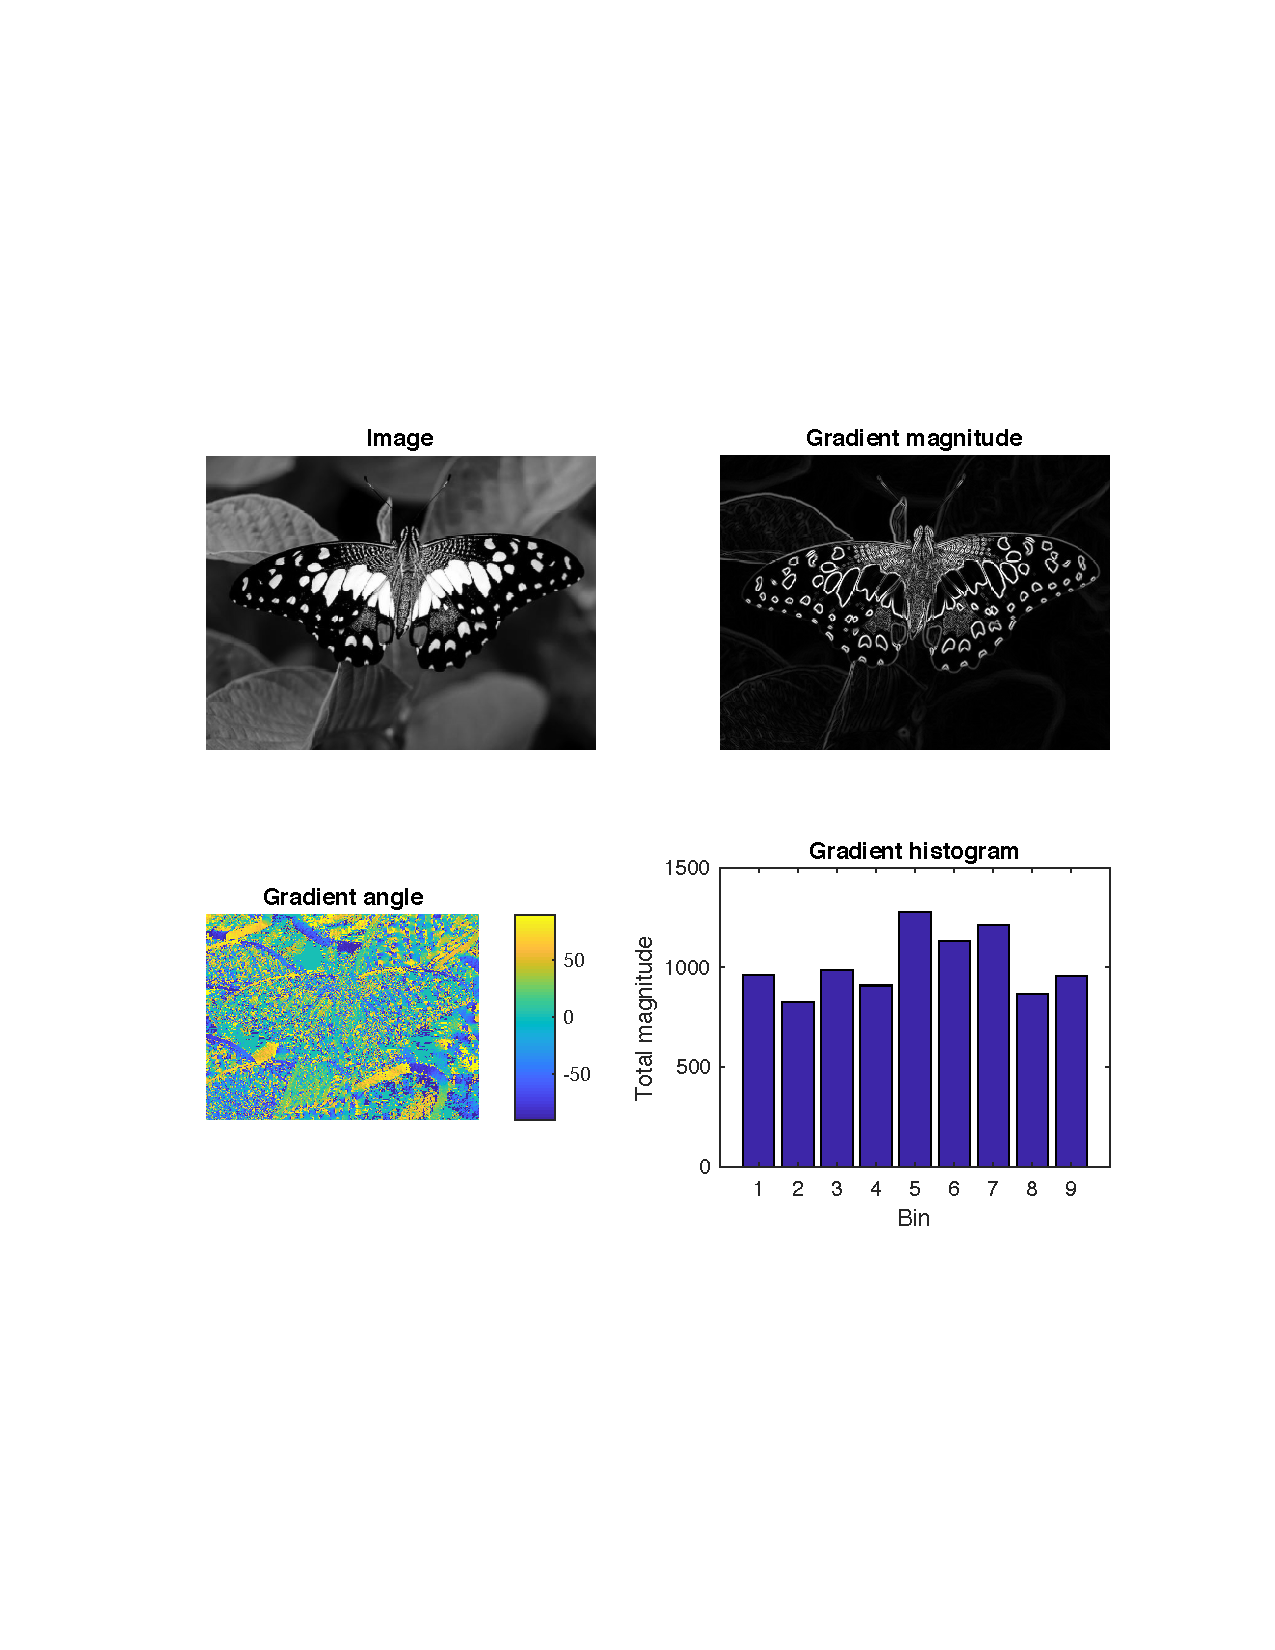
\includegraphics[width=0.9\linewidth]{../latex/figs/butterfly-result.pdf}
\end{figure}
\newpage

\item Visualizing gradient magnitude, angle and histogram for smoothed image
\begin{figure}[h]
\centering
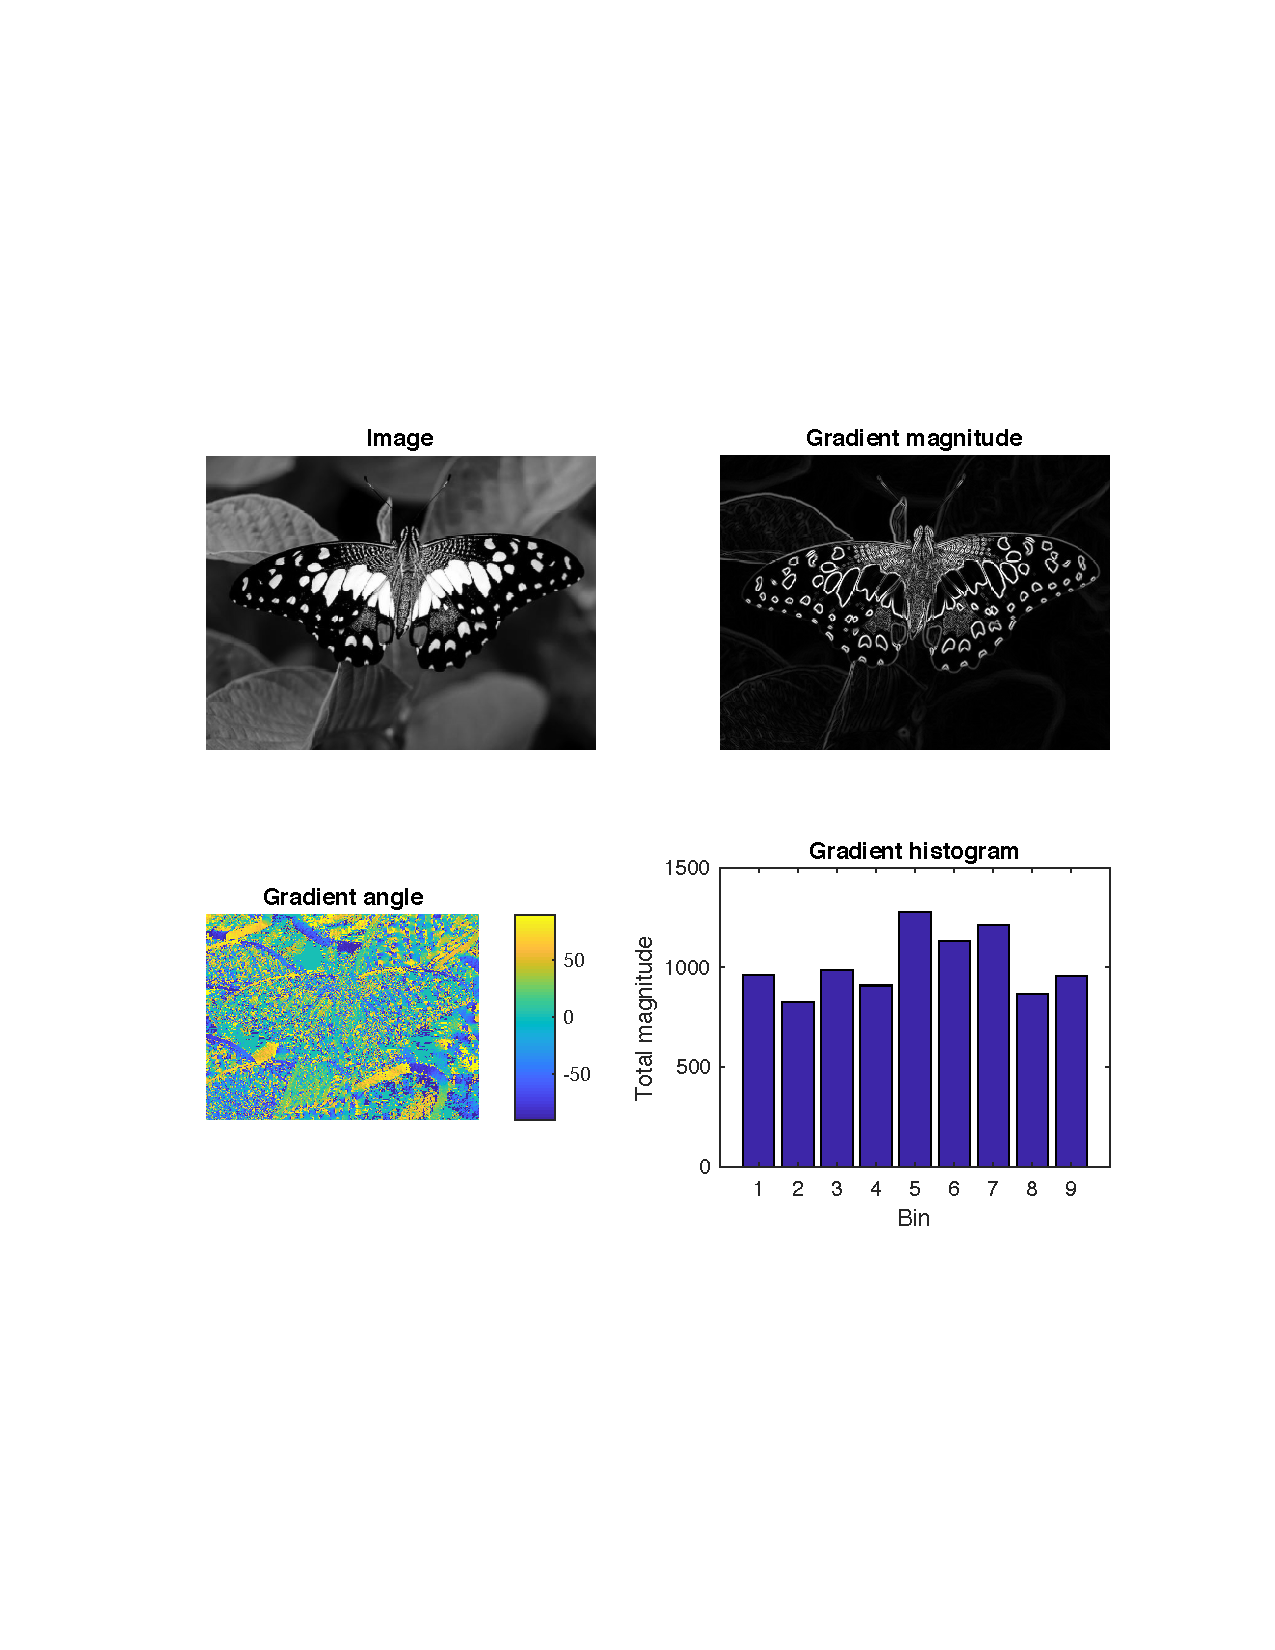
\includegraphics[width=0.9\linewidth]{../latex/figs/butterfly-result.pdf}
\end{figure}
\end{enumerate}
\newpage

\section{Corner detection}

\begin{enumerate}
\item Output for the checkerboard image. When you get the correct output of corner detectors, the heatmaps of corner scores should have higher values (more yellowish) around corners and lower (more bluish) elsewhere.

\begin{figure}[h]
\begin{tabular}{cc}
\includegraphics[trim={4cm 8cm 3cm 7cm},clip, width=0.48\linewidth]{../latex/figs/heatmap.pdf} &
\includegraphics[trim={4cm 8cm 3cm 7cm},clip, width=0.48\linewidth]{../latex/figs/heatmap.pdf} \\
 Corner scores as heatmap (Simple) & Corner scores as heatmap (Harris) \\
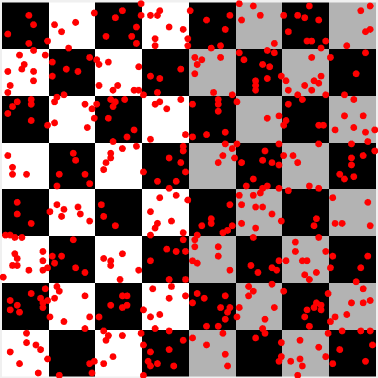
\includegraphics[width=0.48\linewidth]{../latex/figs/checker_simple_corner.png} &
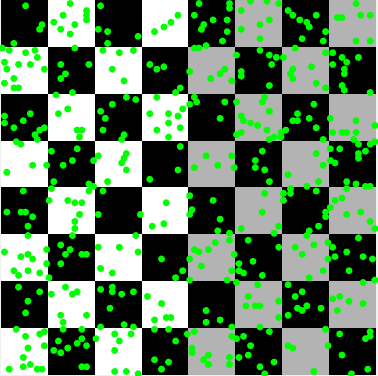
\includegraphics[width=0.48\linewidth]{../latex/figs/checker_harris.png} \\
 Simple corners & Harris corners  \\
\end{tabular}
\caption{\label{fig:checker} Results for the checkerboard image.}
\end{figure}

\newpage

\item Output for the \cmd{'polymer-science-umass.jpg'} image

\begin{figure}[h]
\begin{tabular}{cc}
\includegraphics[trim={3cm 8cm 2cm 7cm},clip, width=0.48\linewidth]{../latex/figs/heatmap_polymer.pdf} &
\includegraphics[trim={3cm 8cm 2cm 7cm},clip, width=0.48\linewidth]{../latex/figs/heatmap_polymer.pdf} \\
 Corner scores as heatmap (Simple) & Corner scores as heatmap (Harris) \\
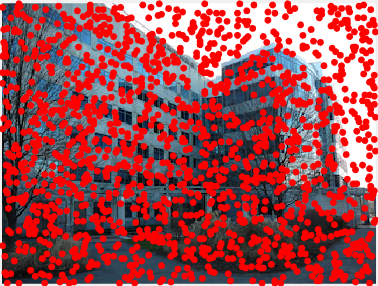
\includegraphics[width=0.48\linewidth]{../latex/figs/polymer_simple_corner.png} &
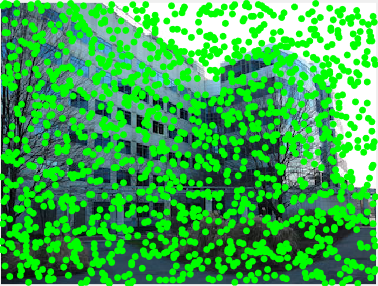
\includegraphics[width=0.48\linewidth]{../latex/figs/polymer_harris.png} \\
Simple corners & Harris corners  \\
\end{tabular}
\caption{\label{fig:polymer} Results for the \cmd{'polymer-science-umass.jpg'} image.}
\end{figure}

\newpage

\item Output for the image of your own choice

\begin{figure}[h]
\centering
\begin{tabular}{cc}
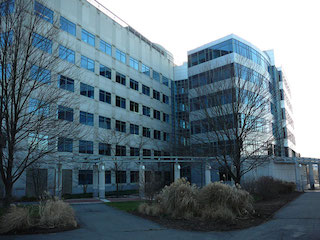
\includegraphics[width=0.48\linewidth]{../latex/figs/polymer-science-umass.jpg} & \\
Input image & \\
\includegraphics[trim={3cm 8cm 2cm 7cm},clip, width=0.48\linewidth]{../latex/figs/heatmap_polymer.pdf} &
\includegraphics[trim={3cm 8cm 2cm 7cm},clip, width=0.48\linewidth]{../latex/figs/heatmap_polymer.pdf} \\
 Corner scores as heatmap (Simple) & Corner scores as heatmap (Harris) \\
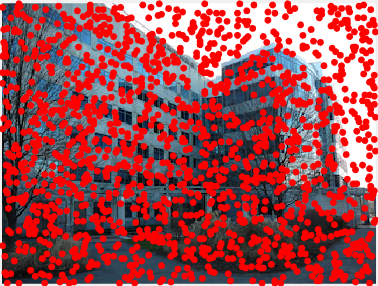
\includegraphics[width=0.48\linewidth]{../latex/figs/polymer_simple_corner.png} &
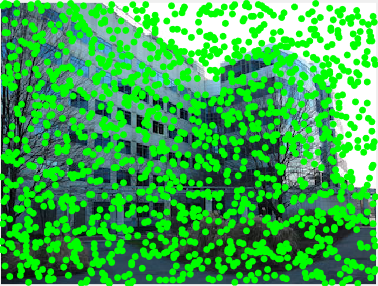
\includegraphics[width=0.48\linewidth]{../latex/figs/polymer_harris.png} \\
Simple corners & Harris corners  \\
\end{tabular}
\caption{\label{fig:own} Results for the image of your own choice.}
\vspace{-2in}
\end{figure}

\end{enumerate}



\newpage

\section{Solution code}
Include the source code for your solutions as seen below (only the files you implemented are necessary). 
In latex the command \cmd{verbatiminput\{alignChannels.m\}} allows you to include the code verbatim as seen below. 
Regardless of how you do this the main requirement is that the included code is readable (use proper formatting, variable names, etc.)
A screenshot of your code works to provided you include a link to source files.



\subsection{detectCorners.m}
\verbatiminput{../initial/detectCorners.m}
\subsection{imageGradient.m}
\verbatiminput{../initial/imageGradient.m}
\end{document}
